\chapter{\textit{Introduction}}
\section{Previous Requirements}
The minimum requirements to run properly the application are:
\begin{itemize} \itemsep0pt \parskip0pt \parsep0pt
	\renewcommand{\labelitemi}{$\rightarrow$}
	\item Operative System: Mac OS X, Windows (XP or newer), Linux, Solaris. 32 or 64 bits architectures.
	\item Software: Java 8 (mandatory requirement).
	\item CPU: AMD or Intel {$>$} 1Ghz.
	\item Memory: At least 512Mb availables.
	\item Graphics Card: AMD/ATI Radeon 9500, NVIDIA GeForce 5 FX, Intel GMA 4500, or better.
	\item Screen: minimun resolution 1024x768
\end{itemize}
\newpage

\section{Application Run}
To run the application it's necessary have installed at least the version 8 of the \textit{Java Virtual Machine} (\emph{http://www.java.com/en/download/}).\\
According to the Operative System installed, can run the application directly from the file explorer or through the system console writing:\\ \emph{java -jar jtlc.jar} over the application folder.
When the application start a new file (\textit{jtlc.settings.props}) is created to store the current settings.
In picture \ref{fig:inicial} is detailed  the application main window.

\begin{figure}[H]
	\vspace{0cm}
	\centering
	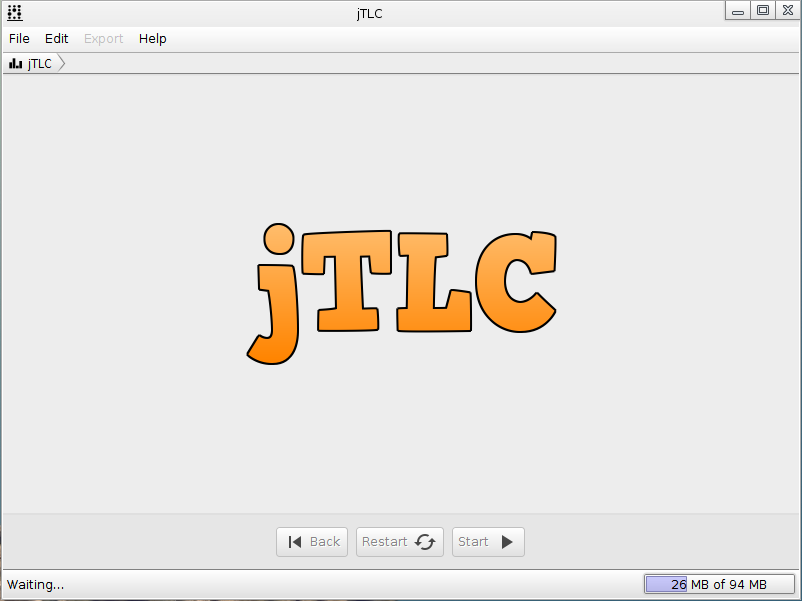
\includegraphics[width=385px]{imagenes/main}
	\centering
	\vspace{-0.4cm}
	\caption{Application initial screen.}
	\label{fig:inicial}
	\vspace{-0.25cm}
\end{figure}
\newpage

\section{Application Settings}
The application settings allows to the user change the system language, projects workspace and enable or disable animations (like screen transition between each analysis screen). To access the settings screen go to \emph{Edit} \ding{222} \emph{Change settings} on the main menu bar.
In the settings screen use \emph{Directory Selector} to change current workspace, the language select to change the application languge, move the animations switch to enable or disable animations. To save current settings click on the button Accept or press \emph{Enter} key from your keyboard. to discard the current settings click on the button Cancel or press \emph{Esc} key.

\begin{figure}[H]
	\vspace{0cm}
	\centering
	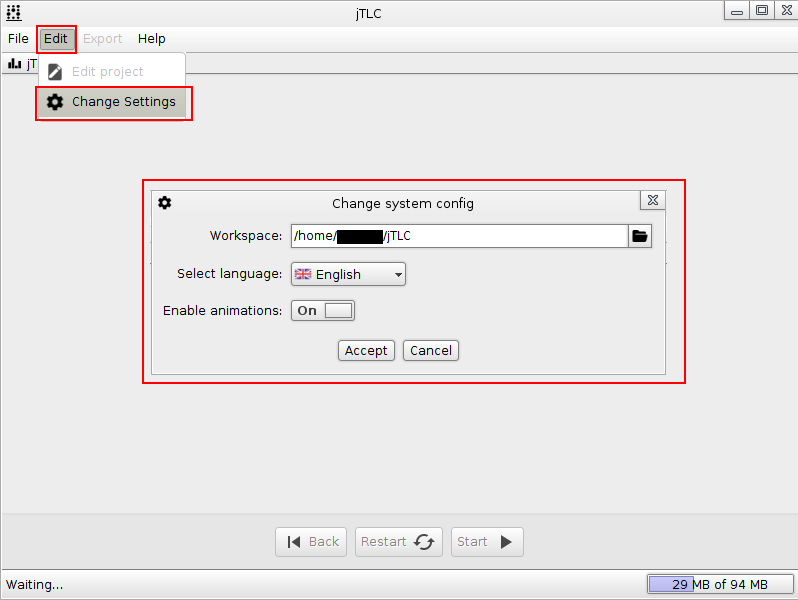
\includegraphics[width=385px]{imagenes/settings}
	\centering
	\vspace{-0.4cm}
	\caption{Application settings.}
	\label{fig:settings}
	\vspace{-0.25cm}
\end{figure}
\newpage

\chapter{\textit{Projects}}
\section*{Start new project}
To start analyzing samples first is necessary start a new project. In the \emph{File} menu use the option \emph{New Project} to create a new project, then the \emph{Create a new Project} dialog will be shown. In this dialog you can introduce the basic information of the project. Click on \emph{Accept} to continue or \emph{Cancel} to abort.
\begin{figure}[H]
	\vspace{0cm}
	\centering
	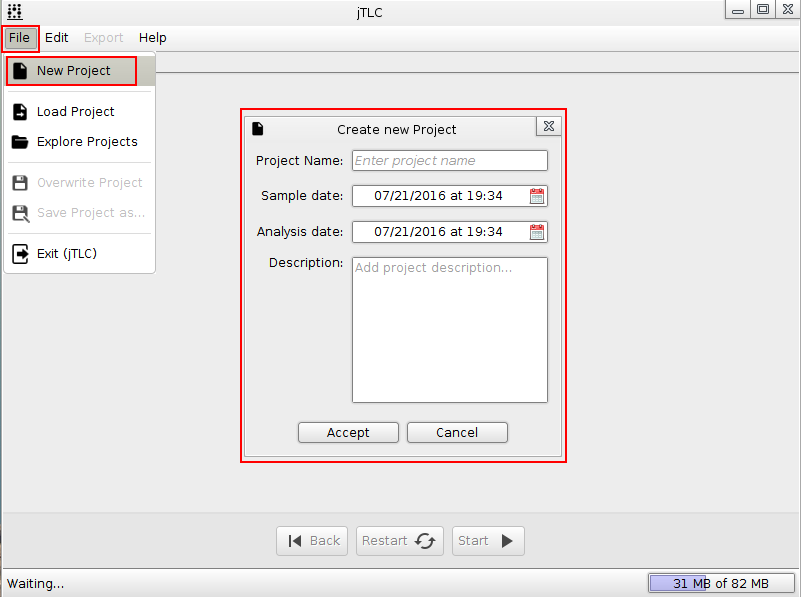
\includegraphics[width=385px]{imagenes/new_project}
	\centering
	\vspace{-0.4cm}
	\caption{New project menu.}
	\label{fig:new_project}
	\vspace{-0.25cm}
\end{figure}
\newpage

\section{Load existent project}
To load a previous project use the option \emph{Load Project} in the \emph{File} menu. A file chooser will be shown where you can select a \textit{jTLC} project file with extension \emph{.jtlc}, select the file and click on \emph{Open} to load or \emph{Cancel} to abort.
\begin{figure}[H]
	\vspace{0cm}
	\centering
	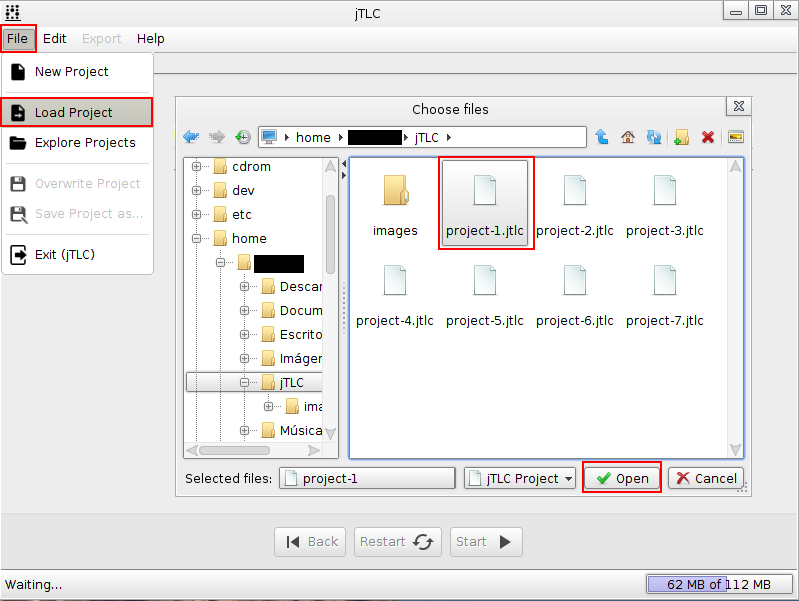
\includegraphics[width=385px]{imagenes/load_project}
	\centering
	\vspace{-0.4cm}
	\caption{New project menu.}
	\label{fig:load_project}
	\vspace{-0.25cm}
\end{figure}
\newpage

\section{Explore projects}
To explore old projects use the option \emph{Explore Projects} in the \emph{File} menu. A directory chooser will be shown where you can select a folder with the \textit{jTLC} project files (\emph{.jtlc} extension), select the folder and click on \emph{Choose} to explore projects or \emph{Cancel} to abort.
\begin{figure}[H]
	\vspace{0cm}
	\centering
	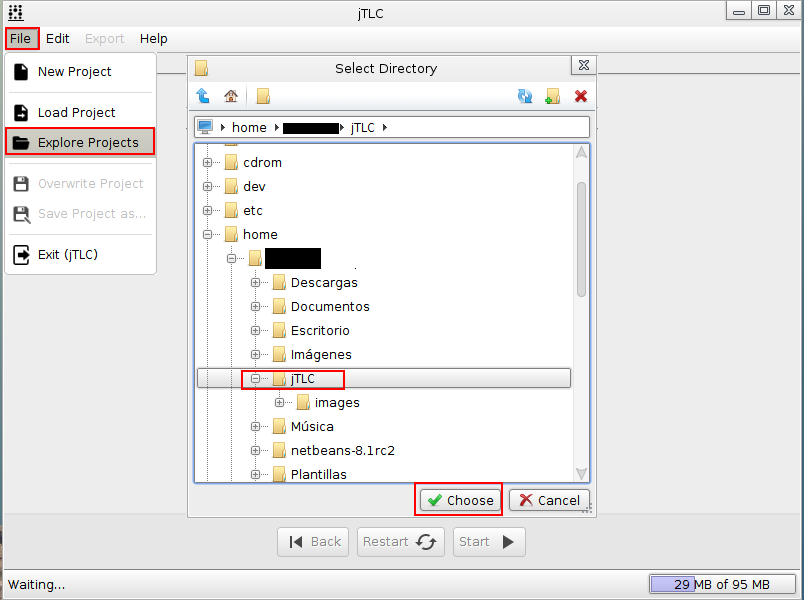
\includegraphics[width=385px]{imagenes/explore_projects}
	\centering
	\vspace{-0.4cm}
	\caption{Explore projects.}
	\label{fig:explore_projects}
	\vspace{-0.25cm}
\end{figure}
\newpage

\subsection{Project Gallery}
After select a folder to explore, the \emph{Project Gallery} will be shown where all the projects in the selected folder are displayed. To view the project details do a click over the project image, the project will be selected as the current project. Use the \emph{arrow keys} Left and Right or use the mouse \emph{scroll wheel} to travel between projects. When a project was selected click on the button \emph{Start} to continue working on that project.
\begin{figure}[H]
	\vspace{0cm}
	\centering
	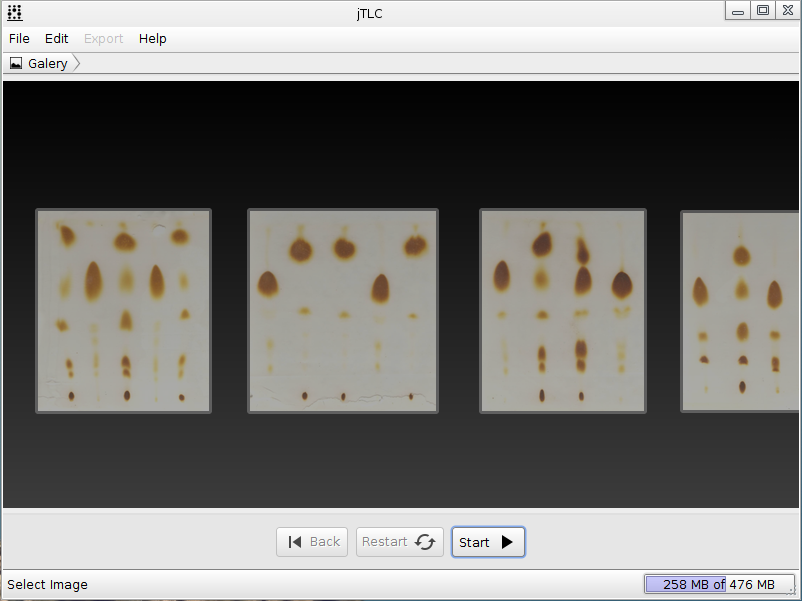
\includegraphics[width=385px]{imagenes/gallery}
	\centering
	\vspace{-0.4cm}
	\caption{Projects gallery.}
	\label{fig:gallery}
	\vspace{-0.25cm}
\end{figure}
\newpage

\section{Edit Project}
To edit the data of current project use the option \emph{Edit project} in the menu \emph{Edit}, a \emph{Edit project data} dialog will be shown where the user can change the project title, description and dates. Use the button \emph{Accept} to save the current values or \emph{Cancel} to abort.
\begin{figure}[H]
	\vspace{0cm}
	\centering
	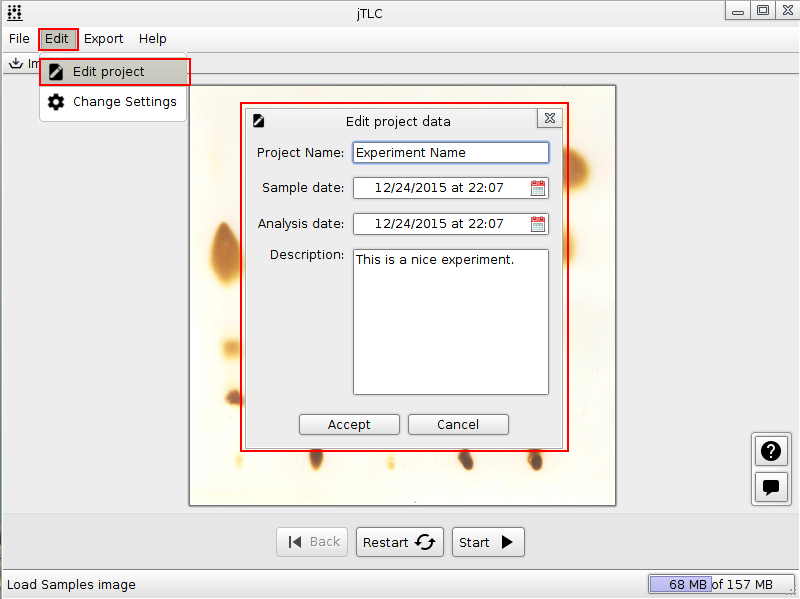
\includegraphics[width=385px]{imagenes/edit_project}
	\centering
	\vspace{-0.4cm}
	\caption{Edit project data.}
	\label{fig:edit_project}
	\vspace{-0.25cm}
\end{figure}
\newpage

\section{Save Project}
To save current project use the option \emph{Overwrite Project}, if exist a previous version (file) of project, or the option \emph{Save Project as...} if it's a new project, in the \emph{File} menu. The option \emph{Overwrite Project} will overwrite the current project file with the new values and data. The option \emph{Save project as...} display a \emph{File Chooser} dialog where you can select a Folder and a File where the project data will be written. Select a File to overwrite/replace or write a new file name (by default it's the project title) and then press the button \emph{Save} to accept or \emph{Cancel} to abort.

\begin{figure}[H]
	\vspace{0cm}
	\centering
	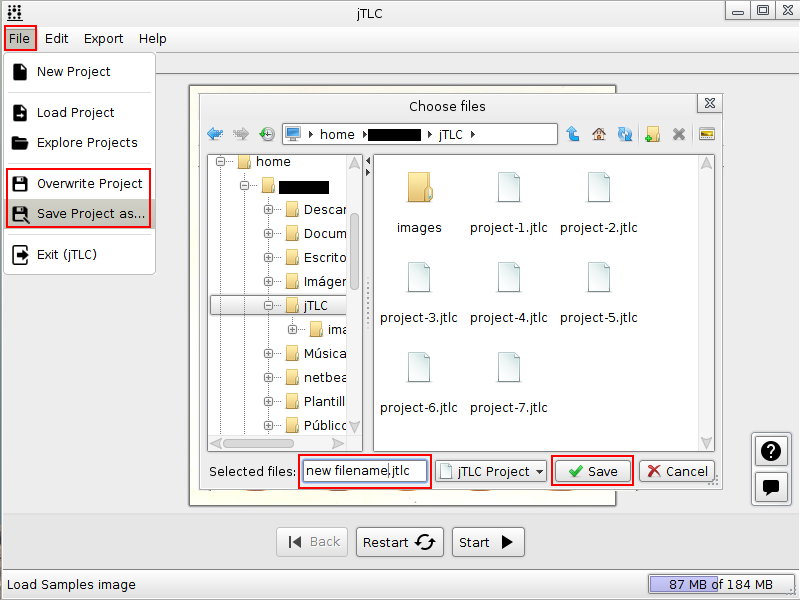
\includegraphics[width=385px]{imagenes/save_project}
	\centering
	\vspace{-0.4cm}
	\caption{Save current project.}
	\label{fig:save_project}
	\vspace{-0.25cm}
\end{figure}
\newpage

\chapter{Samples Analysis}
\section{Image Load}
The first step in the analysis of a sample is to load the image. This task can be performed in two ways. The first is by using the emph\{drag & drop} function, which will allow the user to use the mouse to drag a file to the central area surrounded by dotted lines. The second option allows loading the file is to click on the central area surrounded by dotted lines, which below will open a window that allows the selection of files to search through the files between folders.
\begin{figure}[H]
	\vspace{0cm}
	\centering
	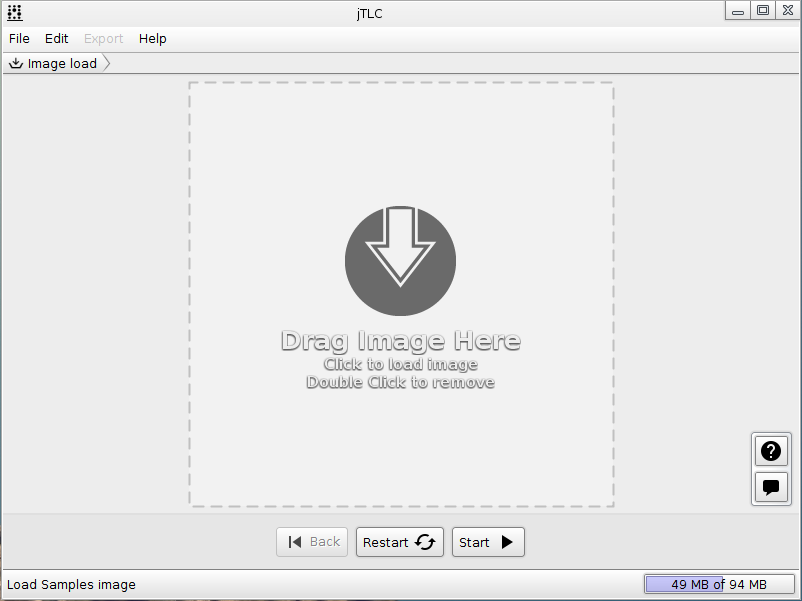
\includegraphics[width=385px]{imagenes/drop}
	\centering
	\vspace{-0.4cm}
	\caption{Load experiment image.}
	\label{fig:image_load}
	\vspace{-0.25cm}
\end{figure}

\section{Image Crop}
Cutting images is done using two sliders, vertical and horizontal, which will allow the cutting lines running from the lateral margins and the upper and lower margins.
\begin{figure}[H]
	\vspace{0cm}
	\centering
	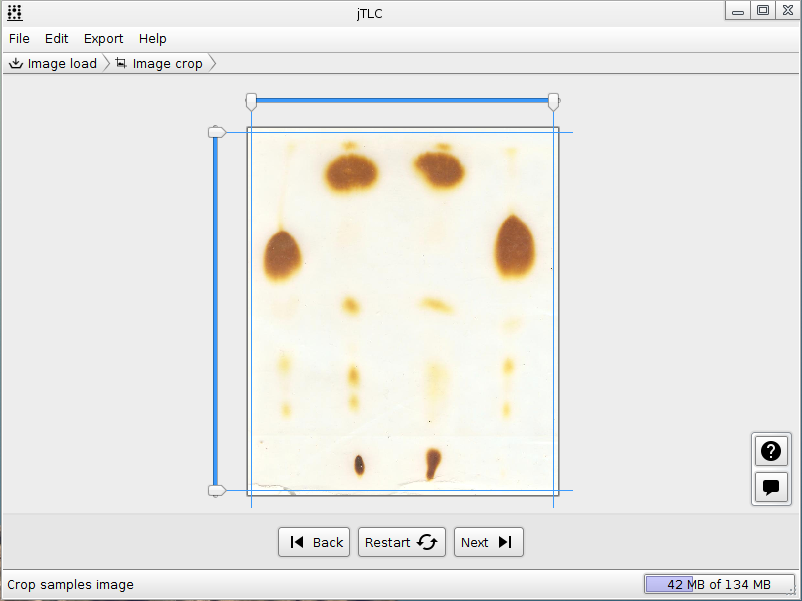
\includegraphics[width=385px]{imagenes/crop}
	\centering
	\vspace{-0.4cm}
	\caption{Crop samples image.}
	\label{fig:image_cut}
	\vspace{-0.25cm}
\end{figure}

\section{Image Rotation}
Esta secci\'on le permite al usuario rotar la im\'agen. Se ofrecen las opciones: \emph{\'angulo de rotaci\'on}, el usuario selecciona el \'angulo preciso a rotar; \emph{girar a la derecha}, gira la im\'agen 90 grados a la derecha; \emph{girar a la izquierda}, gira la im\'agen 90 grados a la izquierda; \emph{invertir verticalmente}, invierte la im\'agen en sentido vertical; \emph{invertir horizontalmente}, invierte la im\'agen en sentido horizontal.
This section allows the user to rotate the image. options are available: \emph{rotation angle}, the user selects the precise angle to rotate; \emph{turn right}, turn the image 90 degrees clockwise; \emph{turn left}, turn the image 90 degrees to the left; \emph{invest vertically} reverses the image vertically; \emph{invest horizontally} reverses the image horizontally.
\begin{figure}[H]
	\vspace{0cm}
	\centering
	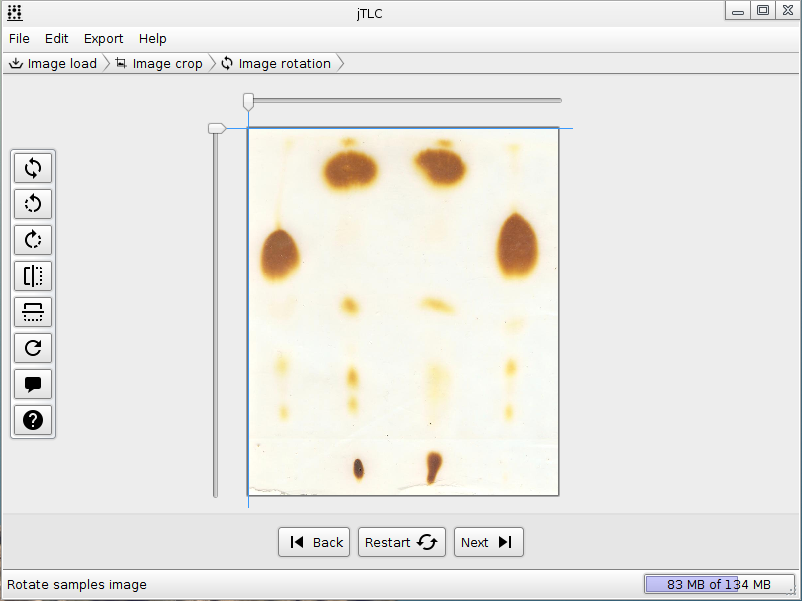
\includegraphics[width=385px]{imagenes/rotate}
	\centering
	\vspace{-0.4cm}
	\caption{Rotate and flip samples image.}
	\label{fig:image_rot}
	\vspace{-0.25cm}
\end{figure}

\section{Samples Selection}
At this stage the user can select a slider samples to be analyzed. In order to submit a sample should be performed double click on the slider while to remove it you must press the \emph{delete} button on the keyboard.
\begin{figure}[H]
	\vspace{0cm}
	\centering
	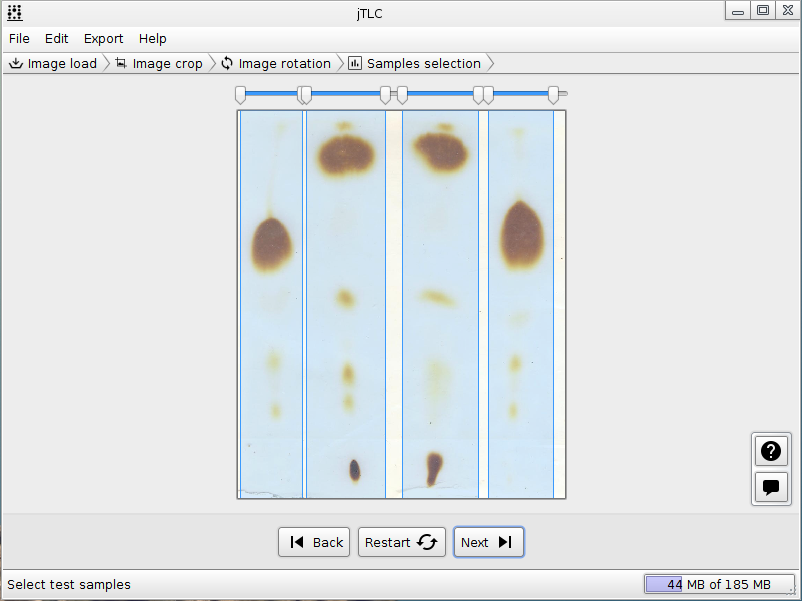
\includegraphics[width=385px]{imagenes/selection}
	\centering
	\vspace{-0.4cm}
	\caption{Individual samples selection.}
	\label{fig:image_samples_selection}
	\vspace{-0.25cm}
\end{figure}

\section{Samples Special Points}
The selection of special points can be done in two ways. The first is individually, while the second allows synchronizing the location of the special points enabling the option to do so under the samples to be aligned together.
\begin{figure}[H]
	\vspace{0cm}
	\centering
	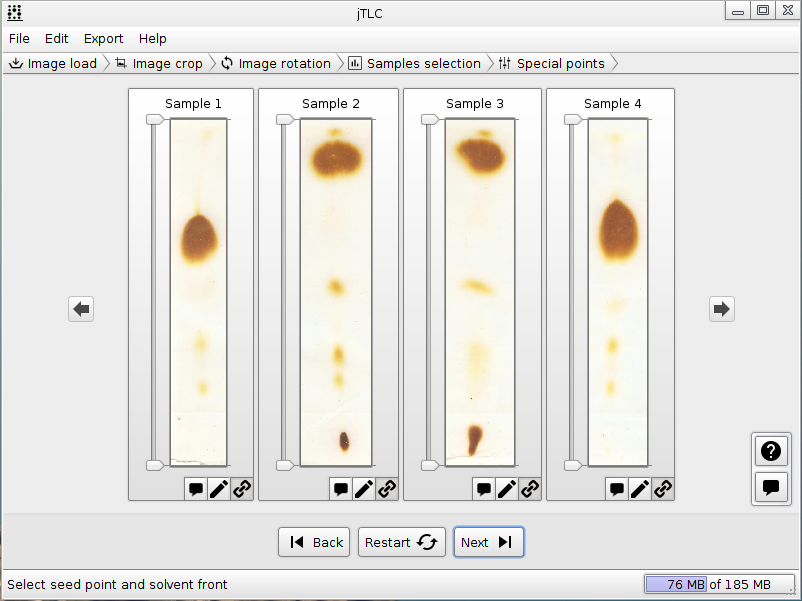
\includegraphics[width=385px]{imagenes/points}
	\centering
	\vspace{-0.4cm}
	\caption{Samples data and special points selection.}
	\label{fig:image_samples_special_points}
	\vspace{-0.25cm}
\end{figure}

\section{Samples Peaks Selection}
One of the final steps is the selection of peaks for each sample. The window is divided into tabs, one for each sample found to exhibit peaks and the user at a time can modify or add similar peaks form when selecting the samples. a slider on the graph and another on the side of the sample is provided, both represent the same sector parallel sample and you can add an area from any of the two options.
\begin{figure}[H]
	\vspace{0cm}
	\centering
	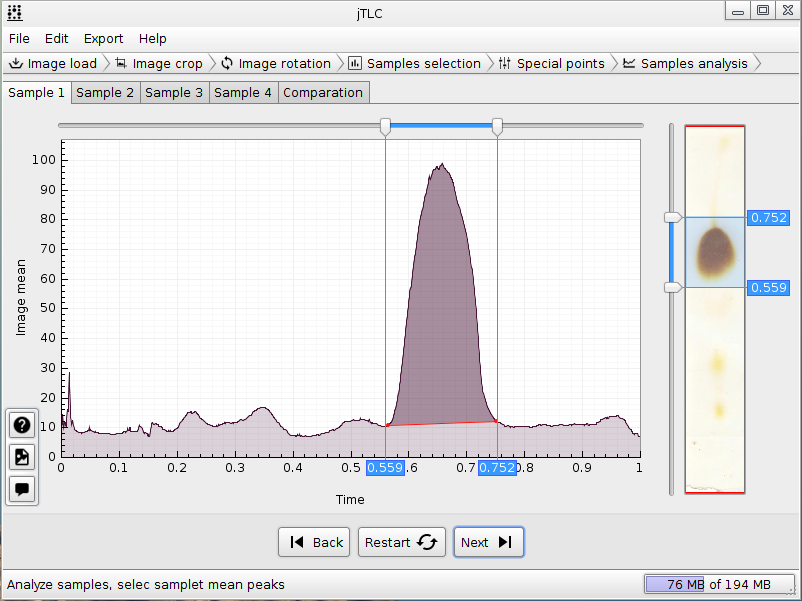
\includegraphics[width=385px]{imagenes/analysis}
	\centering
	\vspace{-0.4cm}
	\caption{Individual samples peaks selection.}
	\label{fig:image_samples_peaks}
	\vspace{-0.25cm}
\end{figure}

\section{Samples Comparation}
At the end of the tab list you can see one that says \emph{comparison} showing all graphics in different colors for each, that color is modifiable and may even remove the transparent fill, or select which samples seen in the comparison .
\begin{figure}[H]
	\vspace{0cm}
	\centering
	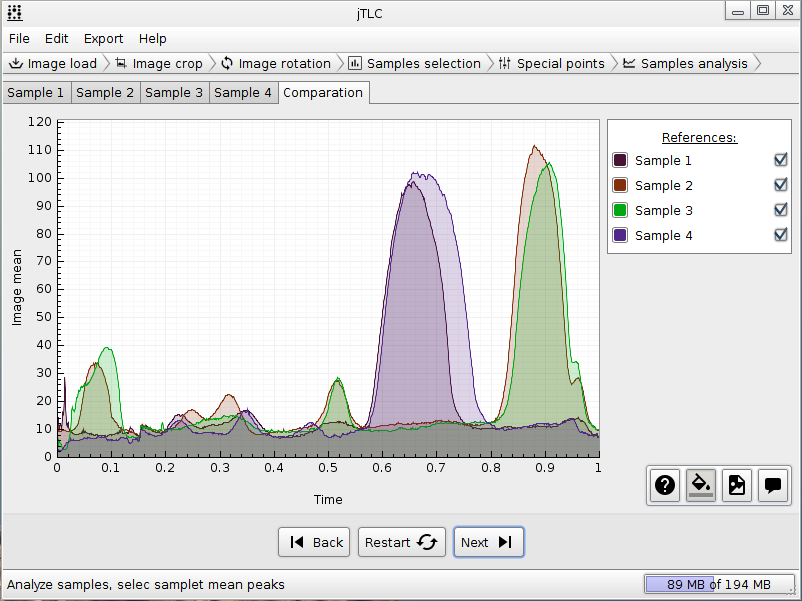
\includegraphics[width=385px]{imagenes/comparation}
	\centering
	\vspace{-0.4cm}
	\caption{Experiment samples mean comparation.}
	\label{fig:image_samples_comparation}
	\vspace{-0.25cm}
\end{figure}

\section{Analysis Results}
De forma an\'aloga a la fase anterior, se muestran los resultados para cada muestra con informaci\'on del an\'alisis realizado en cada pico: l\'imites, m\'aximo, m\'inimo, altura, superficie, superficie relativa y l\'inea  base. Adem\'as se ofrece la opci\'on para exportar la im\'agen de la gr\'afica.
\begin{figure}[H]
	\vspace{0cm}
	\centering
	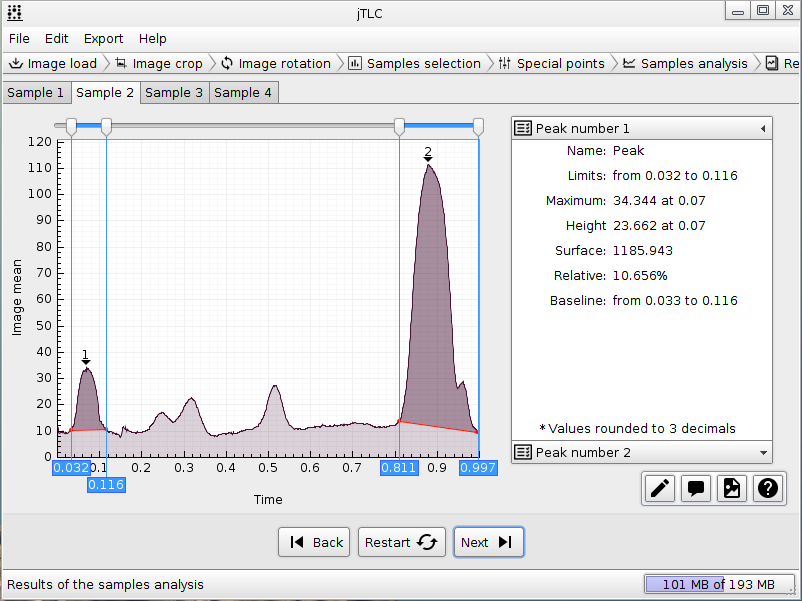
\includegraphics[width=385px]{imagenes/peaks}
	\centering
	\vspace{-0.4cm}
	\caption{Samples peaks analysis results.}
	\label{fig:image_analysis_results}
	\vspace{-0.25cm}
\end{figure}

\section{Analysis Reports}
Again, it using the tabbed window, the information of each sample in report form with all the information, and processed initial images shown. Also shown in the first tab, General project information along with the image containing all samples.
\begin{figure}[H]
	\vspace{0cm}
	\centering
	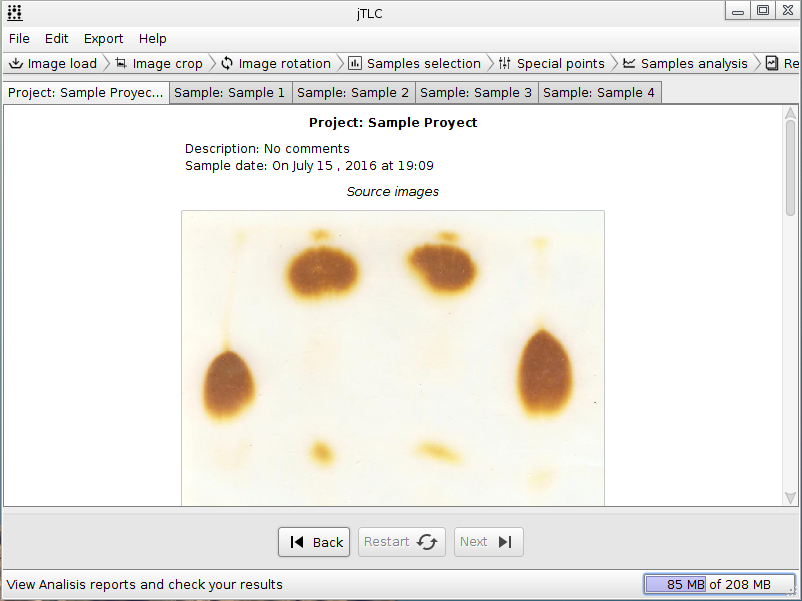
\includegraphics[width=385px]{imagenes/reports}
	\centering
	\vspace{-0.4cm}
	\caption{Samples analysis reports.}
	\label{fig:image_analysis_reports}
	\vspace{-0.25cm}
\end{figure}

\chapter{Data Export}
\section{Export images}
To export the images that worked on the application you must select the \emph{export} option, then, between action lists offered by the popup menu should be selected \emph{original images} which will offer as a result are the initial images: the initial image containing all the sample and the individual samples. Each image after being selected is displayed in a pop-up window with the ability to resize it before choosing which is the directory where you want to save the image.
Another option offered by the \emph{export} menu is \emph{processed image}, which offers the same images of the first option but with the process of trimming and image rotation applied.
\section{Export reports}
To export project information must select the option to \emph{export} and in the menu of options to choose \emph{Reports}. The options available at this point are to export project data or individual samples. At the same time, on each option to export are allowed to decide on the format of the document to export: PDF, ODT, HTML or CSV.
The option to export the project, provides complete information on it. That is, original and modified image, angle correction comments on draft, cutoffs cutout image and cutoffs to separate the samples. Next, it is shown consecutively on each individual sample information (such data are those that can be exported individually). The data displayed on each individual sample are the original images, processed images, points limit, seeding point, front solvent, image and medium peaks of the sample, absolute area, comments on each step of the project, enumerating peaks : position, limits, maximum, minimum, height, total surface area relative and baseline.
\section{Export data}
\subsection{Export mean}
To export information about the mean of each sample should use the \emph{export} option, then select the sample \emph{mean} and which is to extract the information; next step, a text file is downloaded with the requested data.

\subsection{Export plain data}
This option allows you to export in plain text documents, information about the project name, comments and additional data (dates and changes to the original image). When you select a particular sample location information of special points, comments, limits, area, height, maximum, minimum and peak base line shown.